\documentclass[10pt]{article}
\usepackage[ugly]{thesis}

\begin{document}
\pagestyle{plain}
\title{\rmfamily\normalfont\spacedallcaps{Decision
Problems in Invertible Automata}} \author{\spacedlowsmallcaps{Evan
Bergeron \& Klaus Sutner}} \date{May 5, 2017}

\maketitle

\begin{abstract}
  We consider a variety of decision problems in groups and semigroups
  induced by invertible Mealy machines. Notably, we present proof that
  the automorphism membership problem in decidable in these
  semigroups. In addition, we prove undecidability of a Knapsack
  variant. A discussion of iteration and orbit rationality follows.
\end{abstract}

\tableofcontents

\section{Introduction}
The word problem is a classic group-theoretic decision problem. Given
a finitely generated group $G$, and a word $w$ over the generators
(and their inverses), the word problem asks ``is $w \in G$.'' The word
problem is known to be undecidable in surprisingly small classes of
groups - see \cite{Cain09:auto_sg} and \cite{Cain09:dec_prob} for background.

The invertible Mealy machines we consider here give rise to a class of
semigroups (and sometimes groups) for which the word problem is
decidable. The computability picture here is rather nuanced,
however. Similarly important decision problems, among them the
conjugacy problem, and the isomorphism problem are known to be
undecidable - see \cite{sunic:conj} and TODO for details.

We present proof that, for the Abelian case, automorphism membership
testing is decidable in this class of semigroups.

Invertible automata have recently been usefully applied the group
theory. A classic result here is Grigorchuk's group of intermediate
growth, generated by the 5 state invertible machine shown in figure 1.

\begin{figure}
\begin{center}
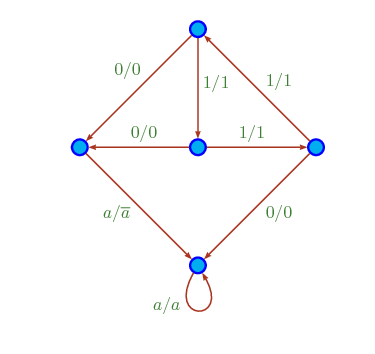
\includegraphics[scale=0.5]{figures/grigorchuk}
\end{center}
\caption{Grigorchuk's 5 state machine}
\end{figure}
\section{Background}
An \defn{automaton} is a formally a triple $(Q, \Sigma, \delta)$,
where $Q$ is some finite state set, $\Sigma$ is a finite alphabet of
\defn{symbols}, and $\delta$ is a transformation on $Q \times \Sigma$.
Automata are typically viewed as directed graphs with vertex set $Q$
and an edge labeled $x \mid y$ between $u, v$ if $(u, x)\delta = (v, y)$.

\begin{center}
\begin{tikzpicture}[
        > = stealth, % arrow head style
        shorten > = 1pt, % don't touch arrow head to node
        auto,
        node distance = 2.5cm, % distance between nodes
        semithick % line style
    ]
    \tikzstyle{every state}=[
        draw = black,
        thick,
        fill = white,
        minimum size = 4mm
    ]
    \node[state] (start) {$u$};
    \node[state] (halt) [right of=start] {$v$};
    \path[->] (start) edge node {$x \mid y$} (halt);
\end{tikzpicture}
\end{center}

One interprets this as if $A$ is in state $u$ and reads symbol $x$,
then $A$ transitions to state $v$ and outputs symbol $y$. A
computation within $A$ may then start at some state $q_0$, and on
input $\alpha_0 \alpha_1 \ldots \alpha_k$, output
$\beta_0 \beta_1 \ldots \beta_k$, where
$(q_i, \beta_i) = (q_{i-1}, \alpha_i)\delta$ for all $i = 0\ldots k$.

As in the above case, where $\delta$ outputs exactly one character for
every transition, we call the automaton $A$ \defn{synchronous}. An
automaton is called \defn{invertible} when every state in $Q$ has some
bijection $\pi$ on $\Sigma$ such that $(u, x)\delta = (v, \pi(x))$. A
state in $A$ is a \defn{copy state} if $\pi$ is the identity
permutation and is a \defn{toggle state} otherwise. The present paper
is concerned only with invertible, synchronous automata.

\subsection{Actions on the infinite tree}

We may identify the set $\Sigma^*$ with an infinite, regular tree of
degree $|\Sigma|$. The root is labelled with the empty string
$\epsilon$, and a vertex labelled $w$ has the child $wa$ for each
$a \in \Sigma$. Out of convenience, we will frequently conflate a
vertex with its label.

% TODO make this less ugly
\begin{center}
\begin{tikzpicture}[
        > = stealth, % arrow head style
        shorten > = 1pt, % don't touch arrow head to node
        auto,
        node distance = 1.5cm, % distance between nodes
        semithick % line style
    ]
    \tikzstyle{every state}=[
        draw = black,
        thick,
        fill = white,
        minimum size = 3mm
    ]
    \node[state] (root) {$\epsilon$};
    \node[state] (s0) [below left  of=root] {$0$};
    \node[state] (s1) [below right of=root] {$1$};
    \node[state] (s00) [below left  of=s0] {$00$};
    \node[state] (s01) [below right=0.56cm and 0.1cm of s0] {$01$};
    \node[state] (s10) [below left=0.56cm and 0.1cm of s1] {$10$};
    \node[state] (s11) [below right of=s1] {$11$};
    \path[->] (root) edge node {} (s0);
    \path[->] (root) edge node {} (s1);
    \path[->] (s0) edge node {} (s00);
    \path[->] (s0) edge node {} (s01);
    \path[->] (s1) edge node {} (s10);
    \path[->] (s1) edge node {} (s11);
\end{tikzpicture}
\end{center}

Each state $q \in Q$ acts on the corresponding tree, sending vertex
$w$ to $wq$. Moreover, if $\alpha \alpha' q = \beta \beta'$, then
$\alpha q = \beta$, for any
$\alpha, \alpha', \beta, \beta' \in \Sigma^*$. Which is to say, $q$'s
action on the tree is an adjacency-preserving map and is thus an
endomorphism on the tree. Since $A$ is synchronous, $q$ is
length-preserving, and thus preserves levels of the tree (and thus is
an automorphism of the tree).

We extend the action of $Q$ on $\Sigma^*$ to words $q = q_1\ldots q_n$
over $Q^+$ by \[ wq = (\ldots((w q_1) q_2)\ldots q_n). \]

This computation corresponds with running $A$ starting at state $q_1$,
then taking that output and running it through the machine starting at
state $q_2$, and so on. We adopt the convention of applying functions
from the right here. In this way, function composition corresponds
naturally with string concatenation.

So there is a natural homomorphism
$\phi : Q^+ \rightarrow \textsf{End}(B^*)$, where $\textsf{End}(B^*)$
denotes the semigroup of endomorphisms of the tree $B^*$. We denote
the image of $\phi$ by $\Sigma(A)$.

\subsection*{Semigroup theory}

A \defn{semigroup} is a set $S$ paired with a binary operation
$f : S \times S \rightarrow S$ such that $S$ is closed under $f$ and
$f$ is associative over $S$. Any set of endofunctions forms a
semigroup under composition.

A semigroup is called \defn{Abelian} when its corresponding binary
operation is commutative.

For an automaton $A$, we denote by $S(A)$ the semigroup generated by
$Q$ under composition. $A$ is said to be \defn{commutative} or
\defn{Abelian} when $S(A)$ is Abelian. We write $G(A)$ for the group
generated by the elements of $Q$ and their inverses.

One may also speak about $S(A)$ and $G(A)$ without explicit reference
to an automaton $A$. As such, we call a semigroup $S$ an
\defn{automaton semigroup} if there is some automaton $A$ with
$S \simeq \Sigma(A)$.
% TODO expand on this
\defn{Automaton groups} $G$ are similarly defined.

\subsection*{Wreath Recursions}
Any automorphism $f$ of $\Sigma^*$ can be written in the recursive form:
\[ f = (f_{\alpha_1}, f_{\alpha_2}, \ldots, f_{\alpha_n})\tau \] where
$n = |\Sigma|$ and each $f_\alpha$ is an automorphism of a subtree of
the root. Here, $\tau$ is some permutation on $\Sigma$. In the case
where $\Sigma = \{0, 1\}$, we have $f = (f_0, f_1)\sigma$ where
$\sigma$ denotes transposition. If $f = (f_0, f_1)\sigma$, $f$ is said
to be \defn{odd}. If $f = (f_0, f_1)$, f is said to be
\defn{even}. That is to say, automorphisms may be classified as even
or odd depending on their action on the first level of the tree.

The endomorphism semigroup of $\Sigma^*$ decomposes into a recursive
wreath product
\[
  \operatorname{End}B^* = \operatorname{End}B^* \wr \tau_\Sigma
\]
where $\tau_\Sigma$ is the tranformation semigroup on $\Sigma$. Which
is to say,
% TODO put the curly underbrace for $n$ times underneath
\[
  \operatorname{End}B^* = (\operatorname{End}B^* \times \ldots \times
  \operatorname{End}B^* ) \rtimes \tau_\Sigma
\]

% TODO running example
% TODO an example here would be very very useful
% TODO residuation maps
% TODO parity maps

% TODO
% Cosets thing

\subsection*{Decision Problems}
Automaton semigroups exhibit many interesting and nuanced
computability properties. While it is an easy result that the
\decprob{word problem} is solvable in such semigroups, similar
group-theoretic problems such as the \decprob{conjugacy problem} and
\decprob{finiteness problem} have been shown to be undecidable
(see \cite{sunic:conj}, and \cite{gillibert:finite}, respectively).

Various other semigroup theoretic decision problems have recently been
considered for small classes of semigroups by Cain in
\cite{Cain09:dec_prob}. We consider a subset of his distinguished
properties in the automaton semigroup case here.

% TODO finitely generated and other background

\section{Decidable Abelian Automorphism Membership}

% TODO definitions of principal automaton, complete automaton, etc

Given an invertible automaton $A$ and a principal Abelian automaton
$B$, we determine if $f = A(p)$ is in the semigroup generated by $B$.

Thus one needs to check if there is some product automaton
\[
  D = B_{p_1} \times B_{p_2} \times \ldots \times B_{p_n}
\]
that implements $f$. We have no computable bound on $n$, so a priori
this merely semidecidable.

Now consider the complete automaton $C$ for $B$, and let $g$ be the
automorphism defined by $D$. After minimization, $D$ produces a
subautomaton of $C$ tat consists of a ``transient part'' and a copy of
$B$ (there may be SCCs in the transient part, but they are not
subautomata). Hence, there is some word $w$ such that $\partial_w g$
is just a single state in the copy of $B$; also, $w$ can be found
effectively\footnote{TODO}. In fact, for all $u$, there is a $w$ such
that $\partial_{ww}g$ is atomic. Essentially this just means that $g$
is strongly tame.

We may safely assume that $A$ is minimal. Then is looks like $A$ has
to have $B$ as a subautomaton to satisfy this ultimate atomicity
condition, plus a transient part sitting on of $B$. It should be
decidable if things match up.

If $B$ is not principal, there are multiple subautomata of $C$ to
content with, but that should not make a major difference. Ditto if
$B$ is just a random subautomaton of $C$.

% TODO
% If same A and r, just identity check.
% If same A, rdifferent r - nontrivial now.
%   - Just a linear subspace problem.
%   - We can assume we have the info up front
%   - Answer is no qne-way and yes the other (bowtie and A32)
% Different A:
%   - Charpoly changes here. Tell you about the identities.
%   - TODO
%   - just write out the equations for the thing you're testing
%
% TODO - come up with two automata with separate A, r, A', r'
%        but there's a function in one machine that can be simulated in the
%        other.

\section{Knapsack is Undecidable for Automaton Semigroups}
% TODO make this formal
We follow a proof strategy similar to \cite{Konig15:knapsack}.

We define the \decprob{Knapsack Problem} as follows: given as input
generators $g_1 \ldots g_k$ and a target semigroup element $g$, do there
exist natural numbers $a_1\ldots a_k$ such that
\[ g_1^{a_1} \cdots g_k^{a_K} = g \] We prove that this problem is
undecidable for automaton semigroups by reducing from % to?
Hilbert's tenth problem.

We define the decision problem \decprob{Hilbert} as following: ``given
a polynomial over the integers and an integer $a$, do there exist
values of the arguments to the polynomial such that the polynomial
evaluated at this point is equal to $a$?'' It is known that there
exist polynomials for which this problem is undecidable.

\textit{Claim: \decprob{Knapsack} is undecidable in the class of automaton semigroups.}

We can expand this polynomial into a system of equations - think of a
codegen step in a compiler. Each step is either an addition or a
multiplication. We can take the terms with negative coefficients and
move them to the other side of the equation, so we now have the
equality of two different polynomials, each with positive
coefficients. We can also choose to only substitute in natural numbers
as arguments, by some trick that I don't know. So then we have systems
of equations over the natural numbers.

We can turn each equation into a formulation of the Knapsack problem
for automaton semigroups. It's known that the Heisenberg semigroup is
an automaton group, and there's some equation over the elements of
$H_3$ for multiplication. Same for addition in the natural
numbers. Then we just take the direct product of these groups (the
class of automaton semigroups is closed under direct product). So this
polynomial is equal to $a$ if and only if there exist $a_1 \ldots a_n$
such that each of the individual elements of the direct product
vectors are equal.

\subsection{A group with decidable word problem with submonoid for
  which the IsGroup question is undecidable}

We define the following ambient group: elements of the group represent
states of a Turing machine. This Turing machine operates on the empty
tape. There is a single halting configuration. In the group, the
element corresponding to the halting configuration is the identity. If
two group elements represent two configurations of the Turing machine
such that one of the configurations can proceed to the other in a
single step, then these two group elements are considered equal.

We have the take care defining the Turing machine, however. We'll
define it to be a \defn{self-verifying} Turing machine. How does this
work? This Turing machine provides some canonical computation, that
is, it proceeds from the start configuration onward, perhaps
halting. However, there are all sorts of configurations that the
Turing machine will never reach. A self-verifying Turing machine will,
at every point, verify that it is along this canonical computation
path. If it finds that it is not, it will transition to some death
state, where it will stay.

This means that, considering the set of all possible configurations of
the Turing machine as a graph, there's a path from the start state
onward (perhaps ending in a halt state) and everything else is just a
star graph transitioning to this death state.

How are these self-verifying Turing machines realized? As the
canonical computation proceeds, a program counter is kept (perhaps to
the left of the tapehead). After every step, the Turing machine will
examine what ``time step'' the computation is currently sitting in. It
will perform the canonical computation for the first $n$ steps. If it
does not wind up where it's configuration says it is, it transitions
to the death state. Otherwise, it continues.

\textit{Claim:} This group has a decidable word problem.

We can verify if one configuration transitions to another in a single
step. So given a word over the generators (that represents a sequence
of TM configurations), we can first go through pairwise, rewriting
these pairs. So I guess chains of consequential configurations just
become their first state. We can also go through and check to see if
certain configurations lie upon the canonical computational path. So
then everything becomes either the death state or the start state or
the identity? Then we can just check for equality of exponents?

\textit{Claim:} If $s$ is the start configuration of the Turing
machine, it is undecidable whether $\langle s \rangle$ is a group.

Suppose it was decidable. We can, given, a TM, transform it into a
self-verifying version of itself, and then build this group around
it. If the original TM halts, then the submonoid generated by $s$,
(the start state) is just the trivial group. If the original TM hangs,
then $\langle s \rangle$ is the free monoid of rank one. So then being
able to answer the question ``is $\langle s \rangle $ a group'' would
allow us to solve the halting problem.

\subsection{It is decidable if an Abelian automaton semigroup
  generates a group}

Reduces to a system of equations. Abelian automaton semigroups can be
written as a system of matrix equations: residuation is a linear
operation here. We can then also write down the set of matrix
equations for the inverse automaton.\footnote{Interesting to note that
  there's some duality here: if the semigroup of $A$ is a group, then
  so is the semigroup of $A^{-1}$ (and they are equal).}  Exactly what
question do we then ask to verify there is a solution? Something about
asking if the space spanned by the equations for $A$ has any
intersection with $\mathbb{N}^n$.

\subsection{Residuation Fixed Point is Decidable for Abelian automaton
  semigroups}

Take the matrix representing residuation for some word
$w \in \Sigma^*$ and find if it has any eigenvectors in
$\mathbb{N}^n$.

\section{Abelian Automata}

\section{Open Questions}

\begin{itemize}
\item All automaton semigroups are recursively presented. If these
  presentations are regular, or context-free, does that affect the
  soluability of these questions?
\item Having a zero
\item Isomorphism problem
\item Bounded automata, etc
\end{itemize}

\nocite{*}\addtocontents{toc}{\protect\vspace{\beforebibskip}}
\addcontentsline{toc}{section}{\refname} \bibliographystyle{plain}
\bibliography{thesis}
\end{document}
